% !TeX spellcheck = de_DE
\chapter{Systemdesign}
\label{sec:design}
Nachdem die Aufgabestellung des Projekts wurde von PSE-Labor veröffentlicht und mit Autorin der Abschlussarbeit besprochen und alle Unklarheiten geklärt, die erste Wahl der Hardware gemacht und die Hardware bestellt wurde und während es auf die Lieferung in das PSE-Labor gewartet wurde, wurde der erste notwendige Schritt angefangen: Systemdesign. Im Rahmen des Systemdesigns werden die Struktur und Zusammenhänge der Elemente des zu entwickelnden Systems untersucht. Das Ergebnis dieser Untersuchung enthält genügend Informationen, um das System zu implementieren. Zuerst wurden die User Stories erstellt. Die sind keine detaillierte Beschreibung der Anforderungen (d.h. was das System tun sollte), sondern eine diskutierte Darstellung der Absicht (Endbenutzer muss/will so etwas tun). Die sind kurz und leicht zu lesen sowohl für Entwicklerin (Autorin) als auch für Stakeholder (mindestens PSE-Labor Mitarbeiter) verständlich. 

Es ist mithilfe der User Stories zu klären, was die zu entwickelnde Datenbank leisten soll. Es wird auf die Frage konzentriert, welche Daten in der Datenbank gespeichert werden sollen. Dazu wird zunächst  die existierende und vorgesehenen Ausleihe-/Rückgabelvorgängen betrachtet und geklärt, welche Informationsobjekte (Personen, Sachen) von Interesse sind und wie diese miteinander in Beziehung stehen. Während der Analysephase wurde auch Sequenzdiagramm erzeugt, die einfach die Interaktionen zwischen Objekten in einer sequentiellen Reihenfolge zeigt, d.h. die Reihenfolge, in der diese Wechselwirkungen stattfinden. Die Sequenzdiagramm wurde als nächstes als eine Basis für das Design des Zustandsmaschine verwendet.  

Für das Systemarchitektur wird das UML-Klassendiagramm entwickelt, das einen Überblick über ein Softwaresystem bietet, indem Klassen, Attribute, Operationen und deren Beziehungen angezeigt werden. Dieses Diagramm enthält den Klassennamen, die Attribute und die Operation in separaten festgelegten Fächern. In der Entwurfsphase wird es festgelegt, welche Klassen das System benötigt wird. Eine Klasse ist eine Vorlage zum Erstellen von Objekten, die Initialisierung von Variablenfeldern und Implementierung des Verhaltens von Feldern und Methoden bereitstellt. Die festgestellte Klassen werden weiter nicht wie üblichen Python-Klassen implementieren, jedoch wie eine Django Modelle direkt zum Erzeugen der Datenbank verwendet. 

\section{Anforderungen und User Stories}
\label{sec:design:user_stories}
Die Softwareentwicklung beginnt normalerweise mit einer Beschreibung der Bedürfnisse und ihrer Analyse. Je genauer und korrekter die Beschreibung der Softwareanforderungen und deren Analyse ist, desto einfacher ist es, alle nachfolgenden Schritte abzuschließen. Das Hauptproblem in dieser Phase ist der Unterschied in den Ansichten des Kunden (in dem Fall der vorliegenden Abschlussarbeit sind die Kunden die PSE-Labor Mitarbeiter) und des Entwicklers (die Autorin der Abschlussarbeit in diesem Fall). Am Anfangs des Abschlussprojekts wurde eine detaillierte Aufgabestellung von PSE-Mitarbeitern geschrieben und auf Beuth Website für die interessierende in der Abschlussarbeiten Studierende veröffentlicht\cite{website:17}. Nachdem die Autorin der Abschlussarbeit auf die Herausforderung achtgegeben hat und mit den PSE-Mitarbeitern bezüglich der Aufgabe kontaktiert, wurde es eine Reihe von Treffen gegeben, während deren haben sich die Kunden (PSE-Mitarbeiter) und die Entwicklerin (die Autorin) sich über die Bedürfnisse der Kunden und die Funktionalität der zu einwickelnde Software geeignet. Es wurde auch die Entscheidung getroffen, mit welchen Hardware ist die Aufgabestellung zu implementieren. Jedoch während der Entwicklung der Register-Client (der einer von drei Bestandsteilen der Software, an dem ein RFID-Leser angeschlossen werden muss), wurde schließlich den RFID-Leser gewechselt. Der Fall ist im Kapitel \ref{sec:register_client:install_rfid} nachzulesen.

Die Analyse der Anforderungen hat sich mit den User Stories angefangen. Eine User Story ist eine Anforderung, die aus der Perspektive eines Endbenutzerziels ausgedrückt wird Sie nehmen keine großen, umständlichen Dokumente auf, sondern sind in Listen gesammelt, die einfacher zu organisieren und neu zu ordnen sind, wenn neue Informationen eintreffen. User Stories werden nicht zu Beginn des Projekts detailliert beschrieben, sondern bereits "just in time" detaillierter entwickelt, um zu frühe Sicherheiten, Verzögerungen bei der Entwicklung, Anhäufung von Anforderungen und eine zu eingeschränkte Formulierung der Lösung zu vermeiden. Sie erfordern wenig oder keine Wartung und können nach der Implementierung sicher abgebrochen werden. Aus der Sicherheitsrunden falls der Festplatte der Rechner der Autorin kaputt geht oder irgendwie anders gehen die Daten die zu einzuwickelnden Software verloren, wird Versionskontrollsystemen namens Git benutzt. Anstatt nur einen einzigen Platz für den vollständigen Versionsverlauf der Software zu haben, wird in Git die Arbeitskopie jedes Entwicklers des Codes auch ein Repository. Das kann den vollständigen Verlauf aller Änderungen enthalten. Während des Corona-Semester, wann den Zugang zum Labor gesperrt wurde und die weitere Kommunikation mit den PSE-Labor Mitarbeitern und Autorin schließlich über Internet geschah, hat Git es auch erlaubt, den Kunden der Software den Fortschritt der Entwicklung zu sehen. 

\begin{figure}
	\centering
	\fbox{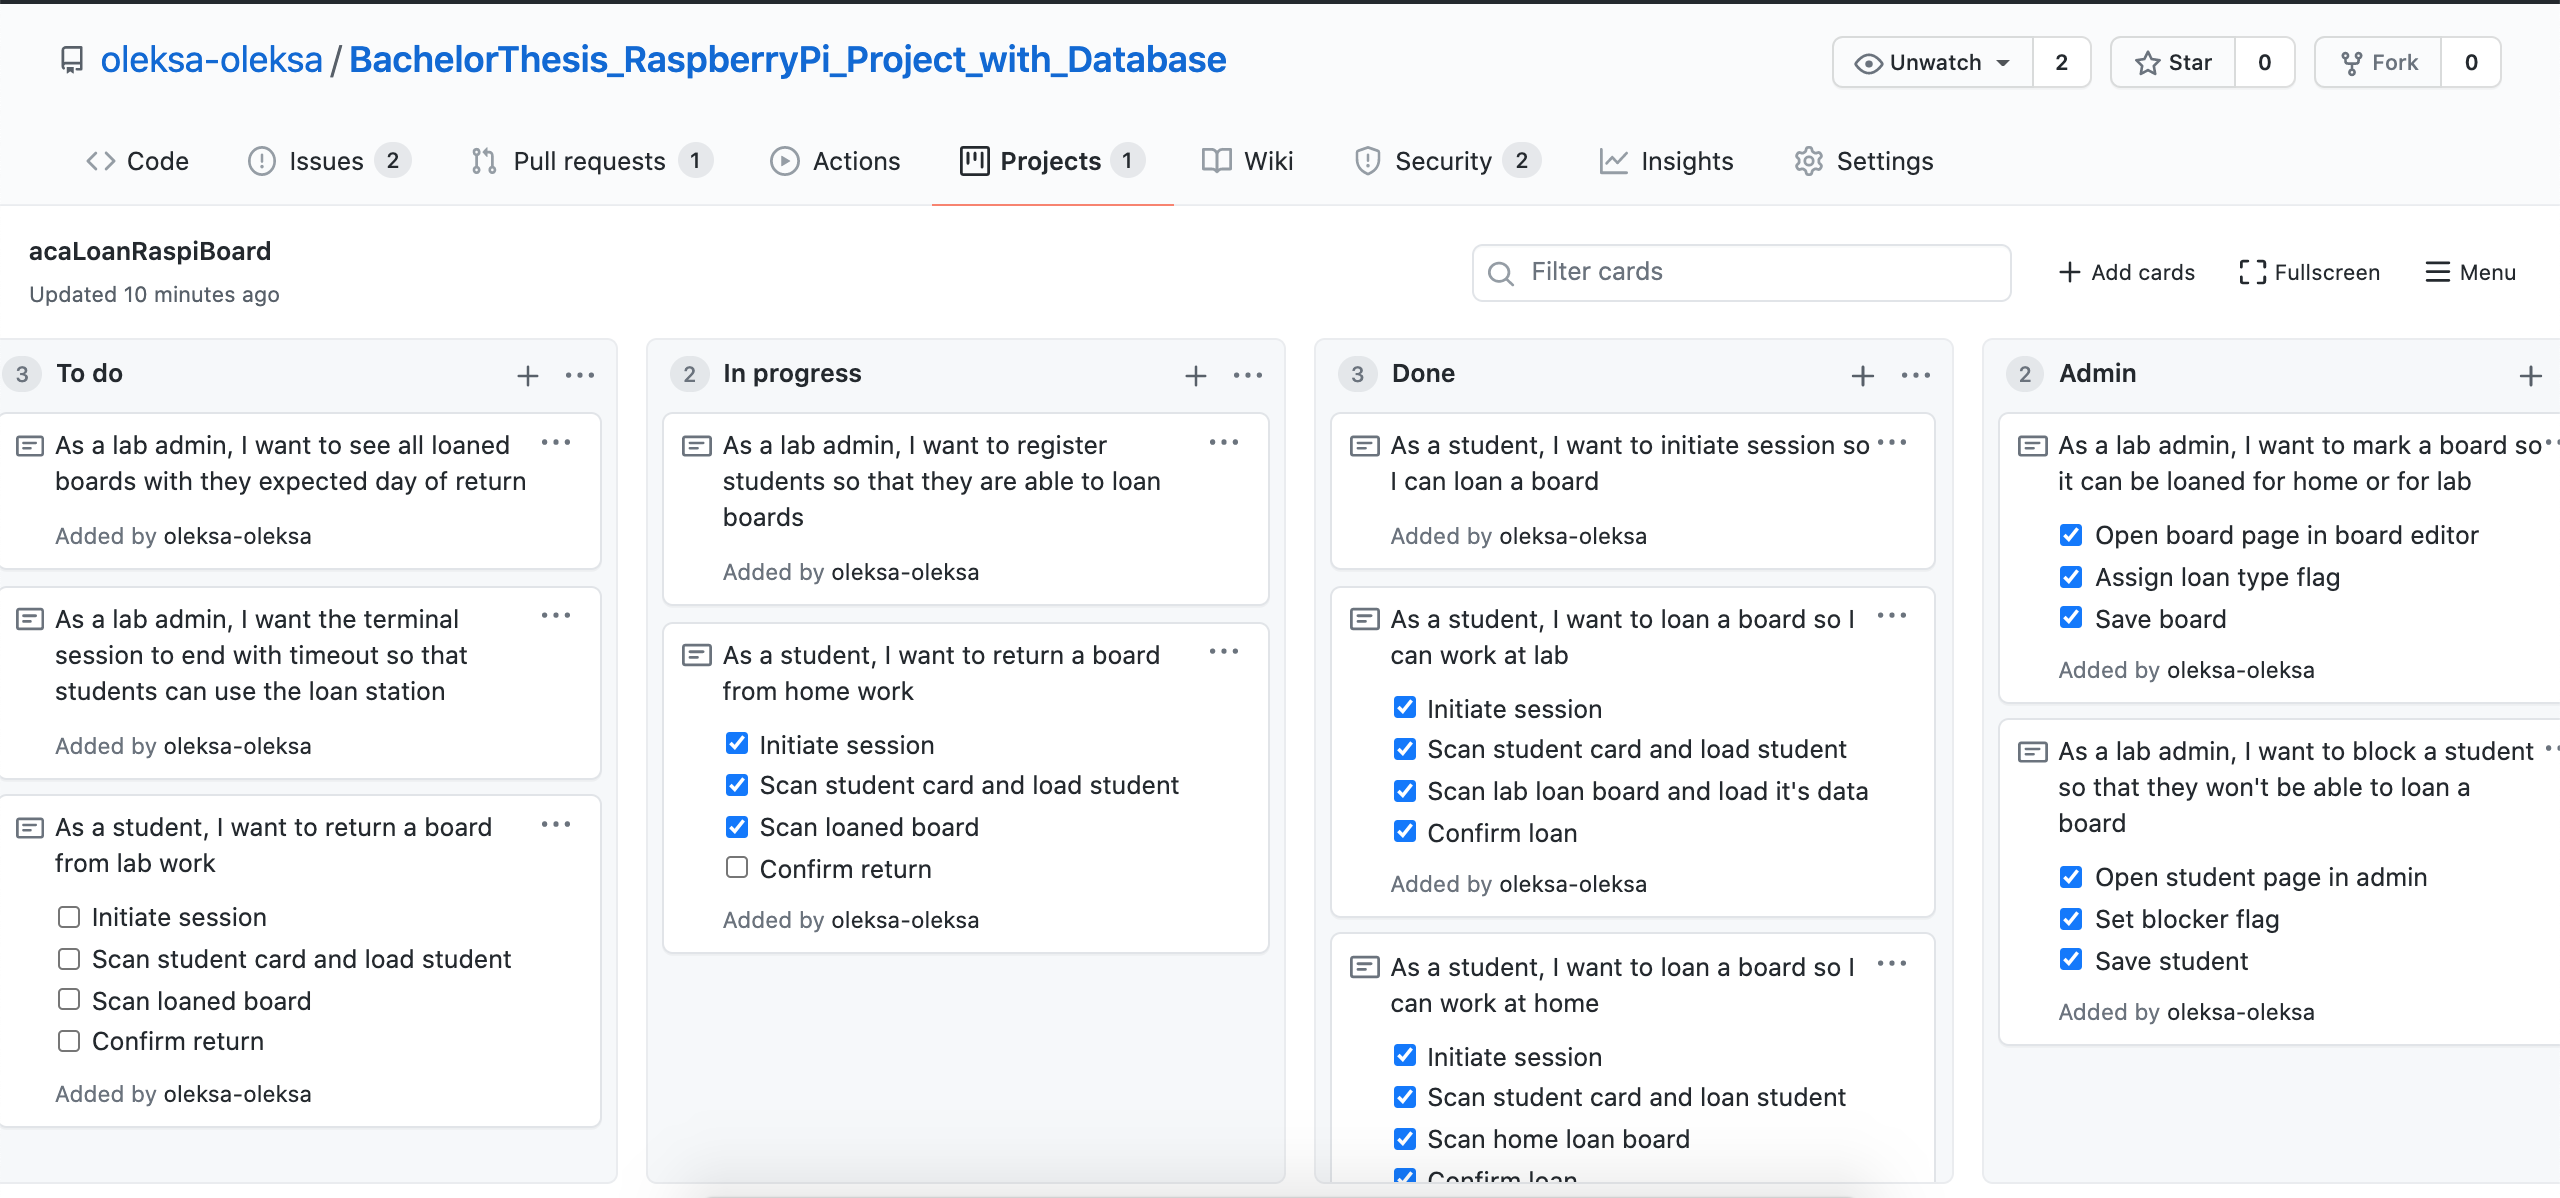
\includegraphics[width=1\textwidth]{gfx/stories.png}}
	\caption{Verwaltung der User Stories auf Github während der Entwicklungsphase}
	\label{fig:stories}
\end{figure}

Seit Oktober 2016 bietet GitHub die Möglichkeit, GitHub-Probleme, Pull-Anfragen und Notizen mit Projekten zu verfolgen. Mit GitHub-Projekten können Boards im Kanban-Stil für die Verwaltung der Arbeit verwendet und separate Code-Repositorys durchschnitten werden. Der Text der User Story selbst sollte die Rolle / Aktionen des Benutzers im System, seine Bedürfnisse und den Gewinn erläutern, den der Benutzer nach dem Auftreten der Story erhält. Zum Beispiel: Wie \textit{<Benutzerrolle / Charakter>, ich <möchte etwas bekommen>, <für diesen und jenen Zweck>}. Es sollte eine Aktion geben - die Hauptaktion. Es macht keinen Sinn, "Autorisieren und Suchen" oder "Suchparameter angeben und eine Suche durchführen" zu beschreiben. Es muss die Aktion angegeben, die Stakeholder wirklich benötigt. Während des Schreibens der User Story wurden zwei Gruppe von Stakeholders definiert für die User Stories geschrieben wurden: die Studierende (Beuth Studentinnen und Studenten) und der Admin (PSE-Labor Mitarbeitern). Es wurden die folgenden User Stories erstellt (als Github Projekt auf der Abbildung \ref*{fig:stories} zu sehen), die später während der Entwicklungsphase implementiert wurden:
\begin{itemize}
	\itemsep-1.2em 
	\item As a student, I want \textbf{to loan a board} so I can work at lab
	\item As a student, I want \textbf{to loan a board} so I can work at home
	\item As a student, I want \textbf{to list boards assigned to me} so that I am sure I to return
	\item As a student, I want \textbf{to return a board from lab work} so that I can loan again
	\item As a student, I want \textbf{to return a board from home work} so that I can loan again
	\item As a student, I want \textbf{to initiate session} so I can loan a board
	\item As a lab admin, I want \textbf{to mark a board} so it can be loaned for home or for lab
	\item As a lab admin, I want \textbf{to terminal session} with timeout so that students can use the loan station
	\item As a lab admin, I want \textbf{to block a student} so that they won't be able to loan a board
	\item As a lab admin, I want \textbf{to see all students} registered on the course so that I can manage their profiles
	\item As a lab admin, I want \textbf{to see all loaned boards} so that I can know their expected return date
	\item As a lab admin, I want \textbf{to register students} so that they are able to loan boards
	\item As a lab admin, I want \textbf{to register new boards} so that thay can be loaned
	\item As a lab admin, I want \textbf{to delete student's record} when semester ends so that they are not stored anymore in database
\end{itemize}

Während die meisten neuen Funktionen mithilfe der User Stories aus Anwendersicht definiert werden sollten, ist dies nicht immer machbar oder sogar hilfreich, wenn es zu Sicherheitsfunktionen oder Infrastrukturanforderungen kommt, die nicht kundenorientiert sind. Die Anforderungen sind in der Regel mehr detailliert und das Schreiben dauert länger. Diese gehen oft technisch auf die Funktionsweise der Software ein. Diese Details leiten das Entwicklungsteam dann beim Erstellen eines neuen Features oder einer neuen Funktionalität. Es gibt zwei Arten von Anforderungen: eine funktionale Anforderung, die beschreibt, was ein Softwaresystem tun sollte, und eine nicht funktionale Anforderungen, die Vorgehensweise des Systems einschränken sollte. Während der Analysephase wurden die beiden Arten von Anforderungen definiert. Die manche von diese Anforderungen sind in der unten geschriebenen Liste zu sehen.

\textbf{Funktionale Anforderungen}
\begin{itemize}
	\itemsep-1.2em 
	\item The background color for all windows in the application will be white and have a hexadecimal RGB color value of 0x0000FF.
	\item The colors of design guidelines of Beuth Hochschule will be used
	\item The software automatically validates whether a student is able to loan a board for a homework
	\item The software automatically shows the information about boards they already loaned
	\item Student will see their name after they scanned their valid student card
	\item Student will see board's number after they scanned a Raspberry Board
\end{itemize}

\textbf{Nicht funktionale Anforderungen}
\begin{itemize}
	\itemsep-1.2em 
	\item Users must use for the initial login their student card. Moreover, every next login will be done with the same card. 
	\item Students never allowed to loan home board longer than 1 week (7 calendar days). Such attempt should be reported to the security administrator.
	\item Students never allowed to loan lab board longer than 120 minutes. An the end of the exercise admnistrator should be notified it the board was not returned.
	\item Loan process can not be started if a student was not properly registered on the course
	\item Every unsuccessful attempt by a user to loan/return an item shall be recorded on an audit trail.
	\item Only one active session is allowed for loan/return process. No multi-user mode is intended
	\item If the currect session is inactive longer longer than 60s the session will be terminated and should be restarted
\end{itemize}

Wie es zu sehen ist, sind User Stories ein großartiges und notwendiges Werkzeug. Die User Story selbst ist die Verbindung zwischen der menschlichen Wahrnehmung und der technischen Umsetzung. Mithilfe der Anforderungen können die Betriebsfunktionen und Einschränkungen des Systems beschrieben werden, die seine Funktionalität verbessern.

\section{Sequenzdiagramm}
\label{sec:design:sequenz}
Sequenzdiagramme beschreiben, wie und in welcher Reihenfolge die Objekte in einem System funktionieren. Diese Diagramme wird häufig verwendet, um Anforderungen an neue und vorhandene Systeme zu dokumentieren und zu verstehen. Ein Sequenzdiagramm ist so strukturiert, dass es eine Zeitleiste darstellt, die oben beginnt und nach unten abfällt, um die Sequenz der Interaktionen zu markieren. Jedes Objekt hat eine Spalte und die zwischen ihnen ausgetauschten Nachrichten werden durch Pfeile dargestellt. Diese Pfeile werden Lebensliniennotationen genannt und ein Sequenzdiagramm besteht aus mehreren dieser Lebensliniennotationen, die horizontal angeordnet sein sollten. Keine zwei Lebensliniennotationen sollten sich überlappen. Sie repräsentieren sie die verschiedenen Objekte, die während der Sequenz im System miteinander interagieren. Es ist besser kleinere Sequenzdiagramme zu zeichnen, die das Wesentliche des Anwendungsfalls erfassen
anstatt ein Sequenzdiagramm mit mehreren Objekten und Gruppen von Nachrichten zu überladen, die den Leser verwirren. In der Abschlussarbeit werden ein paar Sequenzdiagramme gezeigt, die auf den Abbildungen \ref{fig:seq1}, \ref{fig:seq2} und \ref{fig:seq3} zu betrachten sind.

\section{Systemarchitektur}
\label{sec:design:arch}
Das Klassendiagramm definiert die Objekttypen im System und die verschiedenen Arten von Beziehungen, die zwischen ihnen bestehen. Es bietet eine allgemeine Ansicht einer Anwendung. Diese Modellierungsmethode kann mit fast allen objektorientierten Methoden ausgeführt werden. Eine Klasse kann sich auf eine andere Klasse beziehen. Eine Klasse kann ihre Objekte haben oder von anderen Klassen erben.

\section{Endliche Zustandsmaschine}
\label{sec:design:fsm}
